
Vzhledem k vysokému počtu dat pro jeden kalendářní rok, 
v roce 2022 bylo v databázi evidováno přes 32 milionů záznamů o týkající se shrinků
, jsem se rozhodla provést analýzu na měsíčním výběru dat z tohoto období. Jako zkoumaný měsíc jsem vybrala měsíc říjen, neboť v porovnání s letními měsíci a Vánocemi se v říjnu nevyskytují významné sezónní výkyvy.

% [2602933,
%  2439363,
%  2756406,
%  2618723,
%  2809775,
%  2624598,
%  2462898,
%  2545123,
%  2592480,
%  2712669,
%  2543758,
%  2524416]
% 31233142

Zkoumaná říjnová data obsahují $2\ 712\ 669$ řádků a patnáct sloupců. Každý řádek odpovídá jednomu záznamu v databázi shrinku daného produktu. Sledované údaje ve sloupcích jsou: 
% \subsubsection{Sledované údaje}
\begin{itemize}
    \item ID prodejny, kategorická proměnná,
    \item ID produktu, kategorická proměnná,
    \item datum transakce, kategorická proměnná,
    \item typ shrinku, kategorická proměnná,
    \item L1, kategorická proměnná,
    \item L2, kategorická proměnná,
    \item L4, kategorická proměnná,
    \item L5, kategorická proměnná,
    \item L6, kategorická proměnná,
    \item expirace, kategorická proměnná,
    \item množství, spojitá proměnná,
    \item ztracená nákladová cena, spojitá proměnná,
    \item den v týdnu, kategorická proměnná,
    \item číslo den, kategorická proměnná,
    \item období v měsíci (rozdělení měsíce na pět částí), kategorická proměnná.
\end{itemize}
Původní sloupec datum jsem rozdělila na tři jiné proměnné, a to den v týdnu, číslo dne a období v měsíci a sloupec datum jsem vynechala. Z důvodu vysokého počtu záznamů a odlišné povahy dvou typů shrinků jsem data dále rozdělila na shrinky typu damages a shrinky typu inventory. 


\subsection*{Damages shrinky}
Následující část text bude věnována rozboru dat pro shrinky typu damages.



\subsubsection{Výběr dat}
% výběr dle zastoupení shrinků a kategorií produktů a dle outlierů.

Nejprve jsem graficky analyzovala zastoupení shrinků v závislosti na vybraných proměnných pomocí nástroje Power BI, viz obr. \ref*{obr:rok:g:zastoupeni1}. V návaznosti na zjištěné zastoupení shrinků v datech jsem se rozhodla vybrat pouze ty typy shrinků, které tvoří více jak jedno procento z celkových nákladů (tj. náklady činily alespoň jeden milion korun). Vynechala jsem tedy shrinky s označením 5 až 9 a naopak shrinky 0 až 4 byly ponechány. Obdobně jsem přistupovala k záznamům i z hlediska kategorie produktu úrovně L1, jelikož z grafu je patrné, že majoritní zastoupení mají pouze dvě kategorie, a to kategorie superfresh a fresh produktů. Všechny záznamy se zbylými kategoriemi (HBC, others, nonfood, dry food a tobacco) jsem z datasetu odstranila. Těmito kroky jsem zredukovala původní počet řádků datasetu na $1\ 393\ 223$ řádků.

\begin{figure}[hbtp!]
    \centering
    \captionsetup{justification=centering}
    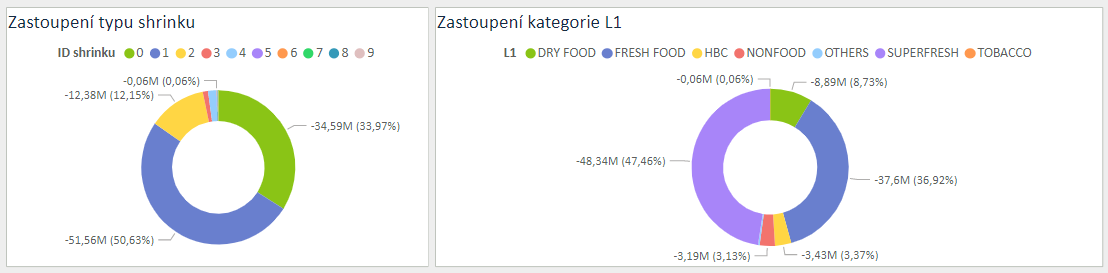
\includegraphics[width=\textwidth]{obrazky/grafy/zastoupeni1.png}
    \caption{Zastoupení shrinků typu damage a zastoupení kategorie L1 v datech \\ z října roku 2022.}
    \label{obr:rok:g:zastoupeni1}
\end{figure}

Jako cílové sloupce (\emph{target} sloupce) jsem určila sloupec s typem shrinku, množstvím produktu a nákladovou cenou. Zbylých jedenáct sloupců slouží jako vysvětlující pro-\linebreak měnné, dále budou označovány jako příznaky pro cílový sloupec. Všechny vybrané příznaky jsou kategorické proměnné, které lze dále rozdělit na nominální a ordinální. Nominální proměnné jsou ID prodejny, ID produktu, kategorie L1, L2, L4, L5 a L6. Ordinální proměnné jsou expirace, den v týdnu, číslo dne a období měsíce. Ordinální příznaky jsem přeznačila tak, aby každá obsahovala pouze hodnoty od nuly do $n_p$, kde $n_p$ je počet kategorií v $p$-tém příznaku. 

Pro další výpočty bylo vhodné přesunout se z nominálních kategorických hodnot na číselné hodnoty. Pro tyto účely jsem zvolila metodu \emph{target encoding}.  %!!! odkaz do teorie, princip meotdy je vysvětlený v kapitole...
Neboť toto kódování na numerické hodnoty zachovává velikost datového souboru, to je klíčové vzhledem k tomu, že nominální proměnné ve zkoumaných datech obsahují velký počet kategorií. Např. počet unikátních produktů v datech je $19\ 026$, což odpovídá stejnému počtu kategorií pro tuto proměnnou. Pokud bych použila one-hot kódování\footnote{One-hot kódování převádí kategorické hodnoty na numerické takovým způsobem že pro každou kategorii vytvoří samostatný sloupec s binárními hodnotami, kde 1 odpovídá dané kategorii a 0 zbylým kategoriím.}  mohlo by dojít k zásadnímu zvýšení počtu sloupců v datech, v tomto případě až o desítky tisíc. \emph{Target kódování} je podobné převodu, který jsem použila pro ordinální proměnné, ale na rozdíl od toho hodnota, která je kategorii přiřazena, souvisí se zastoupením této skupiny v cílovém sloupci a nesouvisí s uspořádáním hodnot uvnitř příznaku. Nevýhodou je, že takto upravená data mohou být náchylná na overfitting, proto je potřeba při predikování použít křížovou validaci.\cite{encoding}

% warehouse_id 339
% product_id 19026
% date_of_transaction 31
% motive_type 10
% cost_value 173409
% L1 7
% L2 20
% L4 141
% L5 450
% L6 1369
% expirace 330
% amount 48634
% weekday 7
% day 31
% quarter_of_month 5

Dále jsem se zabývala identifikací odlehlých hodnot. Nejprve jsem vizualizovala hodnoty pomocí grafu, obrázky \ref*{obr:rok:g:outlierN} a \ref*{obr:rok:g:outlierO}. Z grafu je patrné, že problémová je proměnná $warehouse\_id$, která označuje ID prodejny. Prodejny, které tvoří outliery mohou být malé prodejny, které kvůli menšímu počtu celkových produktů neevidují větší počet shrinků. % !!! jakeho grafu 

\begin{figure}[hbtp!]
    \centering
    \begin{minipage}{.5\textwidth}
        \centering
        \captionsetup{justification=centering}
        
        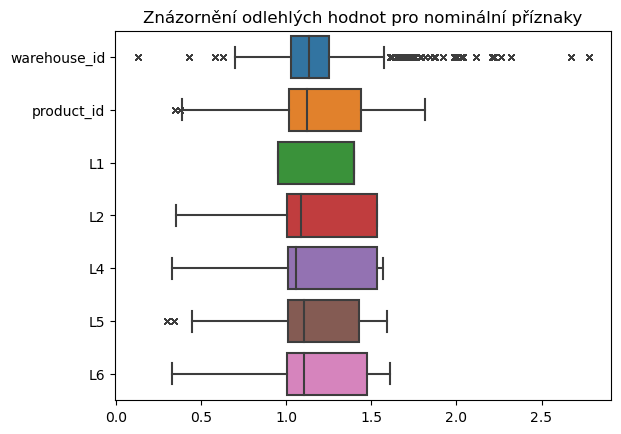
\includegraphics[width=.96\textwidth]{obrazky/zntb/box_nominal.png}
        \caption{Znázornění odlehlých hodnot pro nominální příznaky.}
        \label{obr:rok:g:outlierN}
    \end{minipage}%
    \begin{minipage}{.5\textwidth}
        \centering
        \captionsetup{justification=centering}

        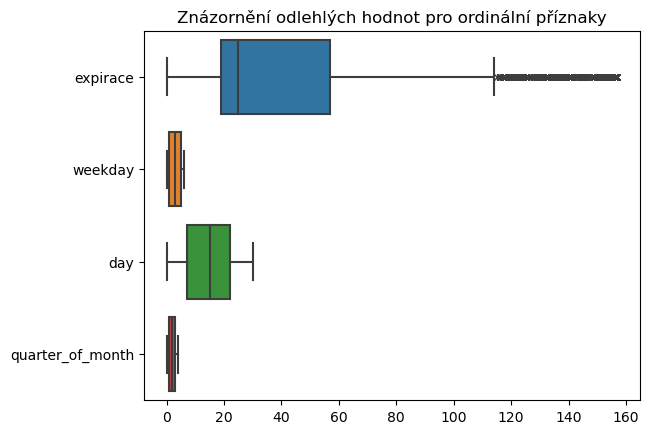
\includegraphics[width=.98\textwidth]{obrazky/zntb/box_ordinal.png}
        \caption{Znázornění odlehlých hodnot pro nominální příznaky.}
        \label{obr:rok:g:outlierO}
    \end{minipage}
\end{figure}

Pomocí Tukeyho testu jsem identifikovala přes $150\ 000$ outlierů pro příznak ID prodejny (\texttt{warehouse\_id}), čímž se dataset zredukoval na $1\ 218\ 453$ řádků. S tímto krokem klesl i počet ostatních outlierů.

V dalším kroku jsem se zaměřila na míru korelace mezi proměnnými. Vizualizovala jsem data pomocí scatter matice pro všechny proměnné, matice je možné vidět na obr. č. \ref*{obr:nb:scatter}. Z této matice můžeme na první pohled vidět, že příznaky odpovídající 4BOX kategorizaci a ID produktu vykazují závislost, což plyne z definice uspořádání této hierarchické kategorizace. V následujících krocích je cílem vybrat tu kategorii, která nejlépe popisuje data ve vztahu k shrinkům.

\begin{figure}[h!]
    \centering
    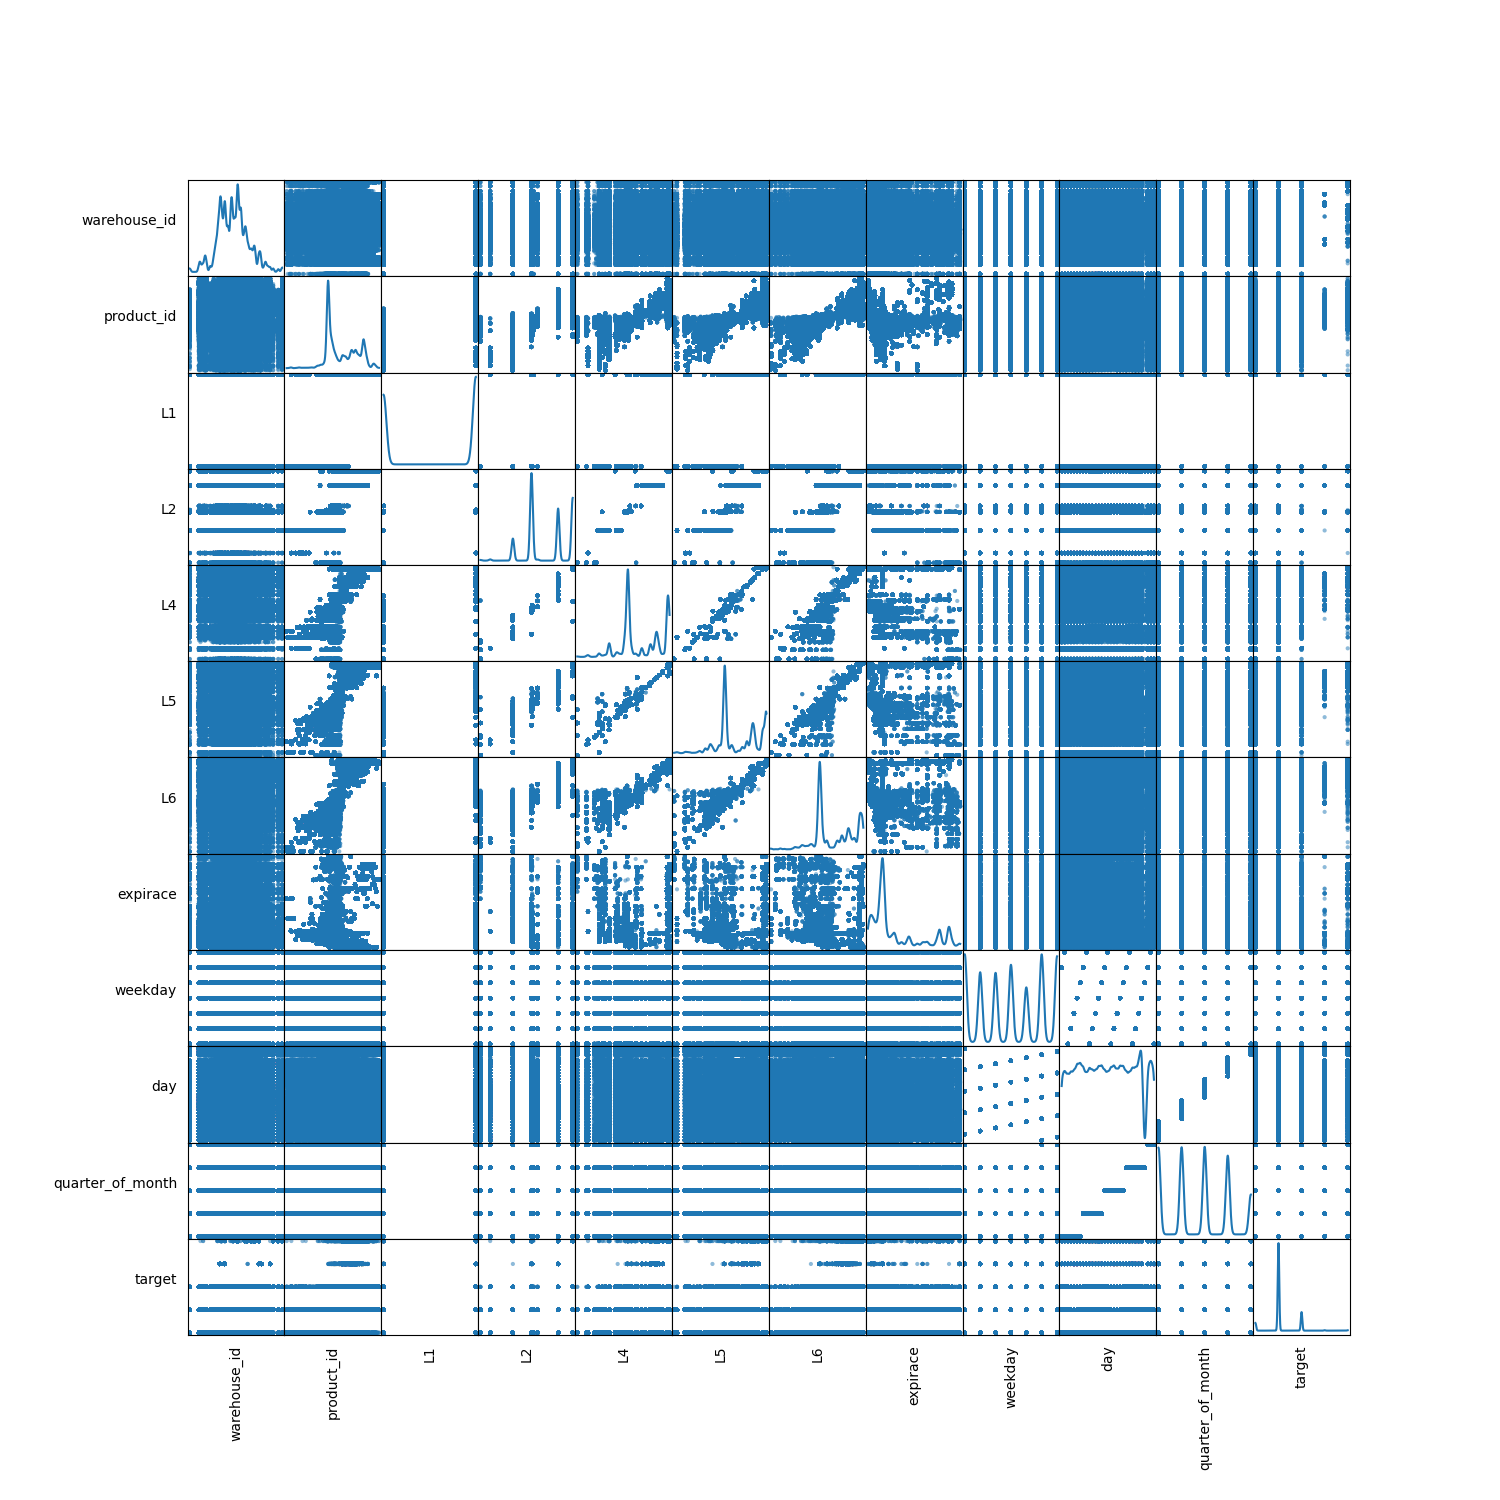
\includegraphics[width=.8\textwidth]{obrazky/zntb/MyScatter.png}
    \caption{Scatter matice příznaků.}
    \label{obr:nb:scatter}
\end{figure}
 
Jako první metodu jsem zvolila $\chi^2$ test. Vzhledem k vysokému počtu dat je matice příliš řídká, a proto nejsou výsledné hodnoty vypovídající a test je tedy pro tuto úlohu nespolehlivý.
Jiným měřítkem pro korelaci mezi proměnnými je Pearsonův korelační koeficient. %!!! odkaz na teorii
Výslednou matici popisující korelační vztahy mezi příznaky jsem vizualizovala teplotní mapou, která je zobrazena na obrázku \ref*{obr:nb:pearson}. Z výsledků je opět patrné, že mezi jednotlivými kategoriemi produktů a produkty je silná korelace. Toto zjištění je zcela logické, neboť se jedná o stromovou strukturu kategorií. Zároveň existuje korelace mezi produktovými kategoriemi a expirací produktu. p-hodnota odpovídající jednotlivým koeficientům byla vždy nulová, kromě pro koeficient týkající se dvojice proměnných expirace a ID prodejny a expirace a pořadí dne v týdnu. Je tedy možné považovat výsledky (kromě těchto dvou výjimek) za statisticky významné.

\begin{figure}[hbtp!]
    \centering
    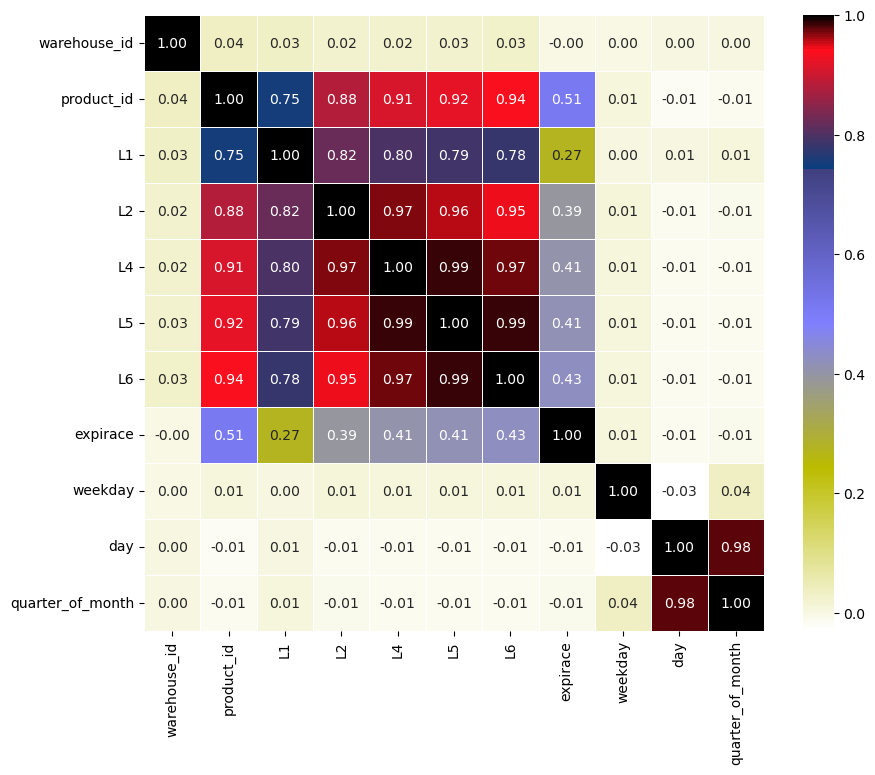
\includegraphics[width=.8\textwidth]{obrazky/zntb/pearson.png}
    \caption{Matice korelačních koeficientů mezi příznaky.}
    \label{obr:nb:pearson}
\end{figure}

Dále jsem použila výpočet koeficientů vzájemná informace \footnote{\emph{mutual information}}, která určuje kolik informace sdílí dvě proměnné. % !!!zdroj
Matice vypočítaných koeficientů je na obr.\ref*{obr:nb:MI}.

\begin{figure}[hbtp!]
    \centering
    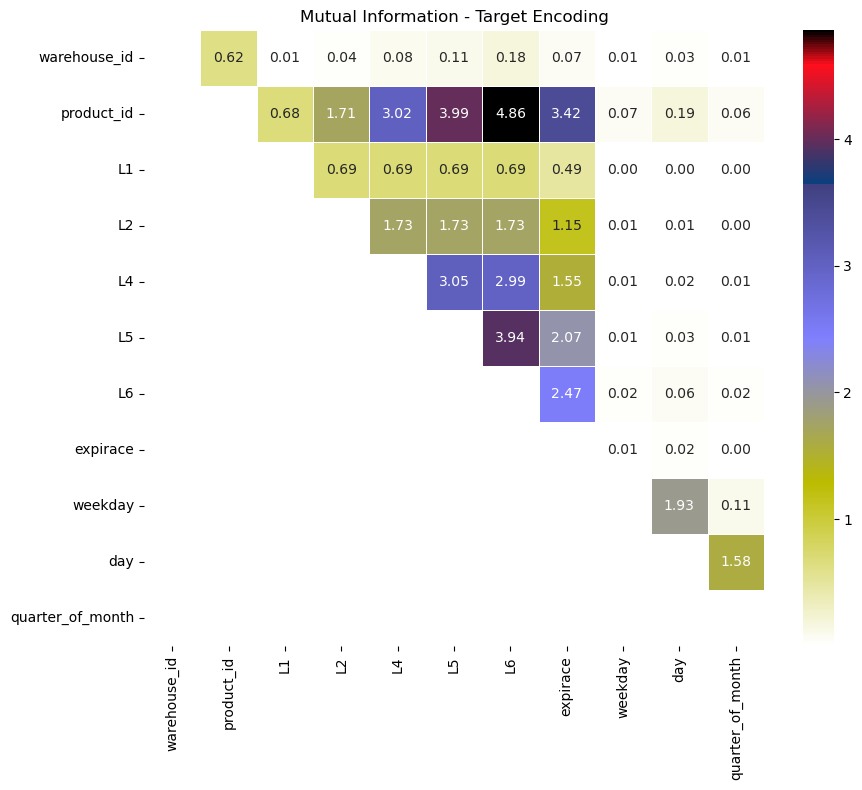
\includegraphics[width=.8\textwidth]{obrazky/zntb/MI_TE.png}
    \caption{Matice koeficientů vzájemná informace mezi příznaky.}
    \label{obr:nb:MI}
\end{figure}

Opět pro znázornění závislosti mezi proměnnými jsem použila koeficient Cramers V a Thiels U. %!!! dopsat co to je %!!!zdroj, odkaz na teorii

\begin{figure}[hbtp!]
    \centering
    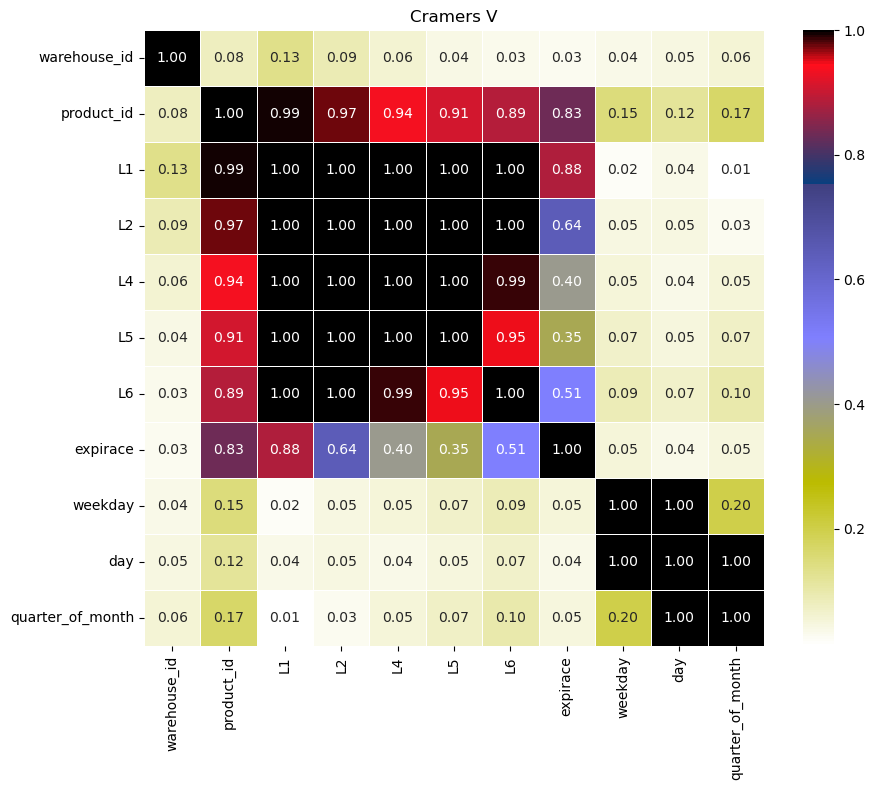
\includegraphics[width=.8\textwidth]{obrazky/zntb/cramers_u.png}
    \caption{Matice koeficientů Cramers U mezi příznaky.}
    \label{obr:nb:cramers}
\end{figure}

\begin{figure}[hbtp!]
    \centering
    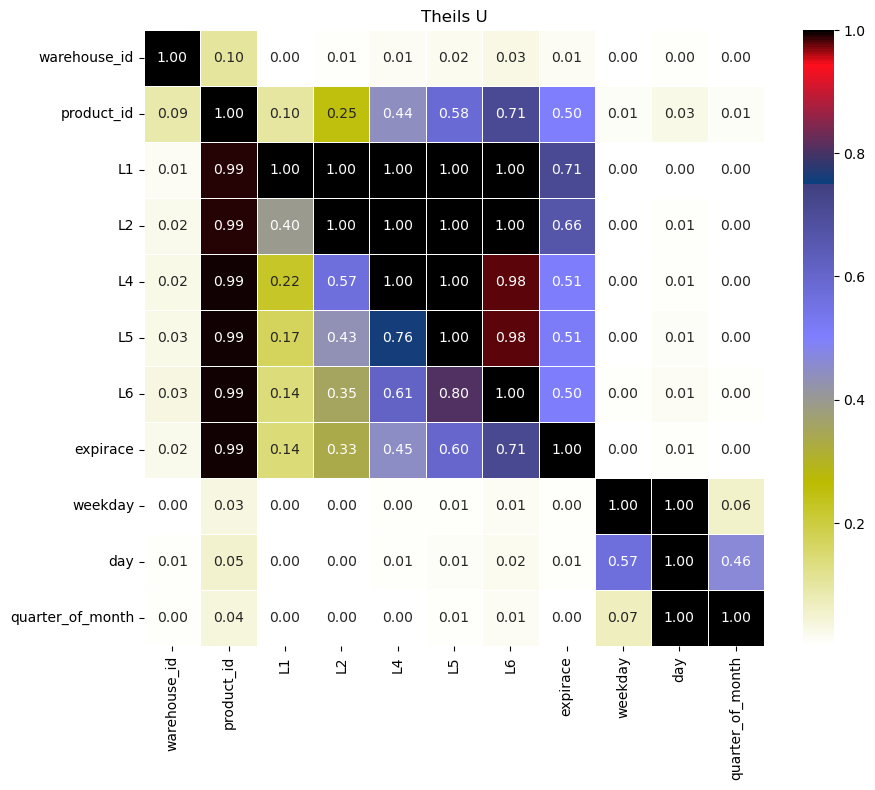
\includegraphics[width=.8\textwidth]{obrazky/zntb/theils_u.png}
    \caption{Matice koeficientů Thiels V mezi příznaky.}
    \label{obr:nb:thiels}
\end{figure}

V dalším testu jsem otestovala multikolinearitu dat pomocí rozptylového inflačního faktoru (VIF). Jako hraniční faktor jsem zvolila hodnotu 40 VIF. Čímž došlo k redukci příznaků z jedenácti na pět na kategorii L1, číslo dne, období měsíce, id prodejny a den v týdnu.

\begin{figure}
    \centering
    \begin{minipage}{.5\textwidth}
      \centering
      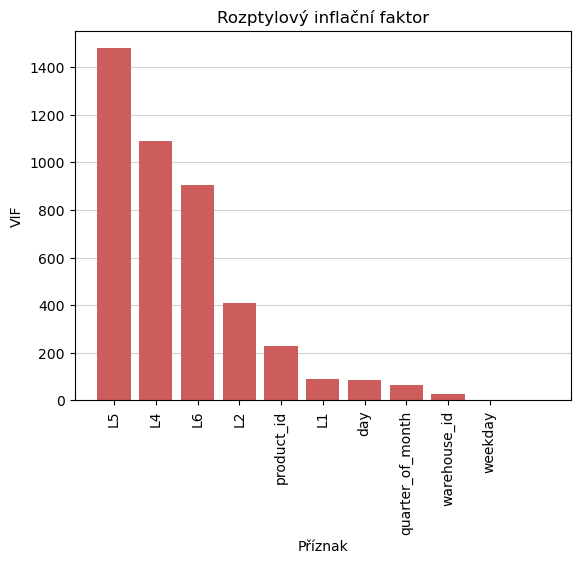
\includegraphics[width=.8\textwidth]{obrazky/zntb/VIF.png}
      \caption{Rozptylový inflační faktor.}
      \label{obr:nb:vif}
    \end{minipage}%
    \begin{minipage}{.5\textwidth}
      \centering
      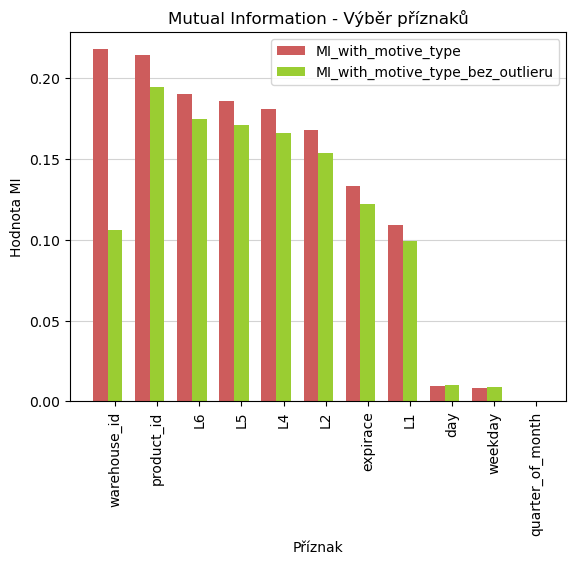
\includegraphics[width=.8\textwidth]{obrazky/zntb/MI_feature_selection.png}
      \caption{Matice koeficientů vzájemná informace mezi příznaky a cílovým sloupcem typ shrinku.}
      \label{obr:nb:MI_FS}
    \end{minipage}
    \end{figure}


Jako další metodu po výběr příznaků jsem vypočítala hodnotu koeficientů vzájemné informace mezi všemi příznaky s target sloupcem. Na obrázku \ref*{obr:nb:MI_FS} lze vidět jak hodnotu jednotlivé proměnné souvisí s cílovým sloupcem.

Potom jsem aplikovala na data analýzu hlavních komponent \ref*{obr:nb:pca_roztyl_komponetn}. Na obrázcích \ref*{obr:nb:pca_roztyl_komponetn} a \ref*{obr:nb:pca_kum_roztyl_komponetn} jsou znázorněny prvních deset komponent a rozptyl který v datech vysvětlují. Na základě hodnot jsem vybrala prvních pět komponent, poté jsem vypočítala příspěvky příznaků k těmto komponentám a vybrala jsem ty příznaky, které příspívají nejvíce - to jsou příznaky id prodejny, den v týdnu, expirace, den a období v měsíci.

\begin{figure}
    \centering
    \begin{minipage}{.5\textwidth}
      \centering
      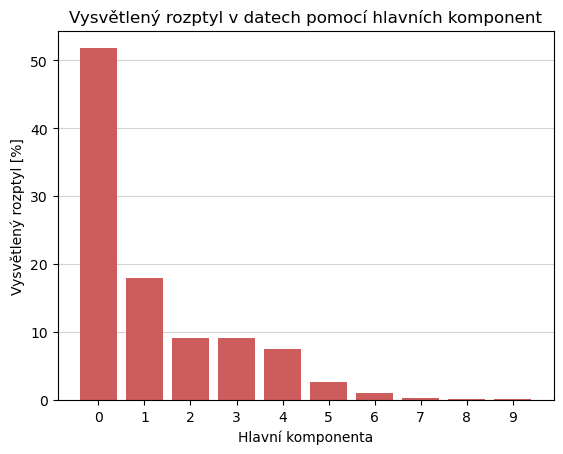
\includegraphics[width=.8\textwidth]{obrazky/zntb/pca-roztyl_komponetn.png}
      \caption{PCA - vysvětlený rozptyl hlavních komponent.}
      \label{obr:nb:pca_roztyl_komponetn}
    \end{minipage}%
    \begin{minipage}{.5\textwidth}
      \centering
      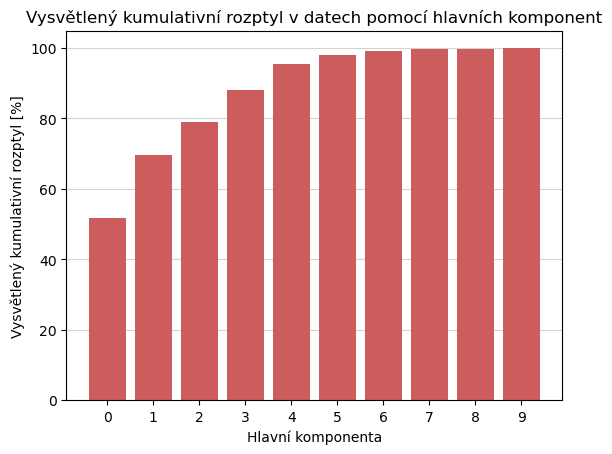
\includegraphics[width=.8\textwidth]{obrazky/zntb/pca-kum_roztyl_komponetn.png}
      \caption{PCA - kumulativní vysvětlený rozptyl hlavních komponent.}
      \label{obr:nb:pca_kum_roztyl_komponetn}
    \end{minipage}
    \end{figure}

\begin{figure}[hbtp!]
    \centering
    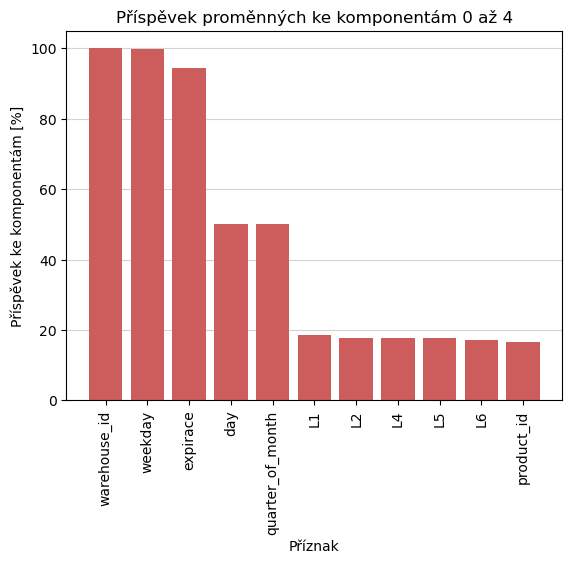
\includegraphics[width=.8\textwidth]{obrazky/zntb/pca-prispevky.png}
    \caption{Příspěvek proměnných ke komponentám 0 až 4.}
    \label{obr:nb:pca_prispevek}
\end{figure}
    